% Source: graduate-coursework/Research/Intro_to_Agents/handouts/Part7_Parallelization.tex

\documentclass[border=4pt]{standalone}
\usepackage{amsmath,amssymb,amsfonts}
\usepackage[T1]{fontenc}
\usepackage{graphicx}
\usepackage{lmodern}
\usepackage{tikz}
\usepackage{xcolor}
\usetikzlibrary{shapes.geometric, arrows.meta, positioning, calc, fit, backgrounds, matrix, decorations.pathreplacing}

\definecolor{UofSCGarnet}{HTML}{73000a}
\definecolor{UofSCBlack}{HTML}{000000}
\definecolor{UofSCWhite}{HTML}{ffffff}
\definecolor{UofSCRose}{HTML}{CC2E40}
\definecolor{UofSCAtlantic}{HTML}{466A9F}
\definecolor{UofSCCongaree}{HTML}{1F414D}
\definecolor{UofSCHorseshoe}{HTML}{65780B}
\definecolor{UofSCGrass}{HTML}{CED318}
\definecolor{UofSCHoneycomb}{HTML}{A49137}
\definecolor{UofSC90Black}{HTML}{363636}
\definecolor{UofSC70Black}{HTML}{5C5C5C}
\definecolor{UofSC50Black}{HTML}{A2A2A2}
\definecolor{UofSCWarmGrey}{HTML}{676156}
\definecolor{UofSCSandstorm}{HTML}{FFF2E3}
\definecolor{UofSCDarkGarnet}{HTML}{570008}
\definecolor{UofSCAzalea}{HTML}{844247}

\tikzset{
    % Node styles - all with sharp corners
    agentbox/.style={
        rectangle,
        draw=UofSCGarnet,
        fill=UofSCSandstorm,
        thick,
        minimum width=2cm,
        minimum height=0.8cm,
        text centered,
        font=\footnotesize
    },
    processbox/.style={
        rectangle,
        draw=UofSCAtlantic,
        fill=UofSCWhite,
        thick,
        minimum width=2.5cm,
        minimum height=0.7cm,
        text centered,
        font=\footnotesize
    },
    syncbox/.style={
        rectangle,
        draw=UofSCCongaree,
        fill=UofSCCongaree!20,
        thick,
        minimum width=3cm,
        minimum height=0.5cm,
        text centered,
        font=\footnotesize\bfseries
    },
    resultbox/.style={
        rectangle,
        draw=UofSCHorseshoe,
        fill=UofSCGrass!30,
        thick,
        minimum width=2cm,
        minimum height=0.7cm,
        text centered,
        font=\footnotesize
    },
    % Arrow styles
    myarrow/.style={
        ->,
        >=Stealth,
        thick,
        UofSCBlack
    },
    dashedarrow/.style={
        ->,
        >=Stealth,
        thick,
        dashed,
        UofSC70Black
    },
    % Timeline styles
    timeline/.style={
        draw=UofSCBlack,
        thick,
        ->,
        >=Stealth
    },
    timeblock/.style={
        rectangle,
        draw=none,
        minimum height=0.5cm,
        text centered,
        font=\tiny
    }
}

\begin{document}
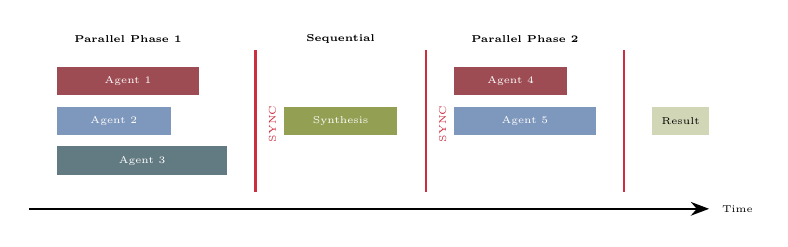
\begin{tikzpicture}[scale=0.72, transform shape]
            % Timeline
            \draw[timeline] (0,0) -- (12,0);
            \node[font=\tiny] at (12.5,0) {Time};

            % Phase 1 - Parallel
            \fill[UofSCGarnet!70] (0.5,2) rectangle (3,2.5);
            \fill[UofSCAtlantic!70] (0.5,1.3) rectangle (2.5,1.8);
            \fill[UofSCCongaree!70] (0.5,0.6) rectangle (3.5,1.1);

            \node[font=\tiny,white] at (1.75,2.25) {Agent 1};
            \node[font=\tiny,white] at (1.5,1.55) {Agent 2};
            \node[font=\tiny,white] at (2,0.85) {Agent 3};

            % Sync barrier 1
            \draw[thick,UofSCRose] (4,0.3) -- (4,2.8);
            \node[font=\tiny,UofSCRose,rotate=90] at (4.3,1.5) {SYNC};

            % Synthesis phase
            \fill[UofSCHorseshoe!70] (4.5,1.3) rectangle (6.5,1.8);
            \node[font=\tiny,white] at (5.5,1.55) {Synthesis};

            % Sync barrier 2
            \draw[thick,UofSCRose] (7,0.3) -- (7,2.8);
            \node[font=\tiny,UofSCRose,rotate=90] at (7.3,1.5) {SYNC};

            % Phase 2 - Parallel again
            \fill[UofSCGarnet!70] (7.5,2) rectangle (9.5,2.5);
            \fill[UofSCAtlantic!70] (7.5,1.3) rectangle (10,1.8);

            \node[font=\tiny,white] at (8.5,2.25) {Agent 4};
            \node[font=\tiny,white] at (8.75,1.55) {Agent 5};

            % Final sync
            \draw[thick,UofSCRose] (10.5,0.3) -- (10.5,2.8);

            % Result
            \fill[UofSCHorseshoe!30] (11,1.3) rectangle (12,1.8);
            \node[font=\tiny] at (11.5,1.55) {Result};

            % Labels
            \node[font=\tiny\bfseries] at (1.75,3) {Parallel Phase 1};
            \node[font=\tiny\bfseries] at (5.5,3) {Sequential};
            \node[font=\tiny\bfseries] at (8.75,3) {Parallel Phase 2};
        \end{tikzpicture}
\end{document}
